 \documentclass{beamer}
%
% Choose how your presentation looks.
% For more themes, color themes and font themes, see:
% http://deic.uab.es/~iblanes/beamer_gallery/index_by_theme.html
%
\mode<presentation>
{
  \usetheme{Madrid}      % or try Darmstadt, Madrid, Warsaw, ...
  \usecolortheme{seahorse} % or try albatross, beaver, crane, ...
  \usefonttheme{serif}  % or try serif, structurebold, ...
  \setbeamertemplate{navigation symbols}{}
  \setbeamertemplate{caption}[numbered]
  \usepackage{amsmath}
  \usepackage{tcolorbox}
  \usepackage[export]{adjustbox}
  \tcbuselibrary{most}
  \usepackage{arydshln}
  \usepackage{tikz}
  \usetikzlibrary{plotmarks}
  \usepackage{pgfplots}
 %\usepackage{enumitem}
%\usepackage{enumerate}
  %\usepackage[shortlabels]{enumitem}
} 


\definecolor{myblue}{RGB}{65,105,225} 
\definecolor{myorange}{RGB}{250,190,0}

\setbeamercolor{structure}{fg=white,bg=myorange}
\setbeamercolor*{palette primary}{fg=myblue,bg=myorange}
\setbeamercolor*{palette secondary}{fg=white,bg=myblue}
\setbeamercolor*{palette tertiary}{bg=myblue,fg=white}
\setbeamercolor*{palette quaternary}{fg=white,bg=myorange!50}

\setbeamercolor{frametitle}{fg=black!90!myblue}

\setbeamercolor{section in head/foot}{fg=white,bg=myblue}
\setbeamercolor{author in head/foot}{fg=black,bg=myorange}
\setbeamercolor{title in head/foot}{fg=white,bg=myblue}

\setbeamertemplate{navigation symbols}{}

\setbeamertemplate{itemize/enumerate body begin}{\large}
\setbeamertemplate{itemize/enumerate subbody begin}{\large}


\defbeamertemplate*{headline}{mytheme}
{%
  \begin{beamercolorbox}[ht=2.25ex,dp=3.75ex]{section in head/foot}
    \insertnavigation{\paperwidth}
  \end{beamercolorbox}%
}%

\defbeamertemplate*{footline}{mytheme}
{
  \leavevmode%
  \hbox{%
  \begin{beamercolorbox}[wd=.5\paperwidth,ht=2.25ex,dp=1ex,right]{author in head/foot}%
    \usebeamerfont{author in head/foot}\insertshortauthor\hspace*{2em}
  \end{beamercolorbox}%
  \begin{beamercolorbox}[wd=.5\paperwidth,ht=2.25ex,dp=1ex,left]{title in head/foot}%
    \usebeamerfont{title in head/foot}\hspace*{2em}\insertshortsubtitle\hspace*{2em}
    \insertframenumber{} / \inserttotalframenumber
  \end{beamercolorbox}}%
  \vskip0pt%
}



\usepackage[english]{babel}
\usepackage[utf8x]{inputenc}
\usepackage{xcolor}
\usepackage{listings}
\usepackage{pgf}  
\usepackage{textpos}
\usepackage{tabulary}
\usepackage{scrextend}
\usepackage{hyperref}
\usepackage{setspace}
\usepackage{rotating}
\lstset
{
    language=[LaTeX]TeX,
    breaklines=true,
    basicstyle=\tt\scriptsize,
    %commentstyle=\color{green}
    keywordstyle=\color{blue},
    %stringstyle=\color{black}
    identifierstyle=\color{magenta},
}
\newcommand{\bftt}[1]{\textbf{\texttt{#1}}}
%\newcommand{\comment}[1]{{\color[HTML]{008080}\textit{\textbf{\texttt{#1}}}}}
\newcommand{\cmd}[1]{{\color[HTML]{008000}\bftt{#1}}}
\newcommand{\bs}{\char`\\}
\newcommand{\cmdbs}[1]{\cmd{\bs#1}}
\newcommand{\lcb}{\char '173}
\newcommand{\rcb}{\char '175}
\newcommand{\cmdbegin}[1]{\cmdbs{begin\lcb}\bftt{#1}\cmd{\rcb}}
\newcommand{\cmdend}[1]{\cmdbs{end\lcb}\bftt{#1}\cmd{\rcb}}

\newcommand{\wllogo}{\textbf{Overleaf}}

% this is where the example source files are loaded from
% do not include a trailing slash
\newcommand{\fileuri}{https://raw.githubusercontent.com/GiancarloSucci/UniBo.IDSEPC.A2022/main/A2022.IDSEPCLaTeX/}


\usepackage{stackengine}
\def\Ruble{\stackengine{.67ex}{%
  \stackengine{.48ex}{\textsf{P}}{\rule{.8ex}{.12ex}\kern.6ex}{O}{r}{F}{F}{L}%
  }{\rule{.8ex}{.12ex}\kern.6ex}{O}{r}{F}{F}{L}\kern-.1ex}



%----------------------------------------------------------------------------------------
%	TITLE PAGE
%----------------------------------------------------------------------------------------
\title[L01]{ {\textit{Corso di Laurea in Governance e Politiche dell'Innovazione Digitale}} \\\\
Sentir, Meditar ... e Programmar(e) -- Data Science e Pensiero Computazionale} % The short title appears at the bottom of every slide, the full title is only on the title page

\author[{\tiny Giancarlo Succi }]{Giancarlo Succi\\\\ Dipartimento di Informatica -- Scienza e Ingegneria\\Universit\`{a} di Bologna\\
\bftt{g.succi@unibo.it}
} % Your name
\institute[unibo] % Your institution as it will appear on the bottom of every slide, may be shorthand to save space

\date{} % Date, can be changed to a custom date

\setbeamertemplate{navigation symbols}{}
\AtBeginSection[]
{
        \begin{frame}<beamer>{Outline}
                \tableofcontents[currentsection]
        \end{frame}
}
\begin{document}
\begin{frame}
\titlepage % Print the title page as the first slide

\end{frame}

%=============================================

\addtobeamertemplate{frametitle}{}{%
\begin{textblock*}{10mm}(-0.01mm,-0.95cm)

\includegraphics[width=0.9cm]{unibo-logo.png}
\end{textblock*}}

%=============================================


\begin{frame}
{\centerline{Sentir, Meditar ... e Programmar(e)}}
\begin{itemize}
    \item La natura del software
    \item La funzione di costo
    \item La lezione di Calvino
\end{itemize} 
\end{frame}

\begin{frame}
{\centerline{Sentir ...  (1/3)}}
\begin{itemize}
    \item Il software \`{e} il risultato di un atto creativo della mente umana
\end{itemize} 
\vspace{0.8cm}
\begin{center}
    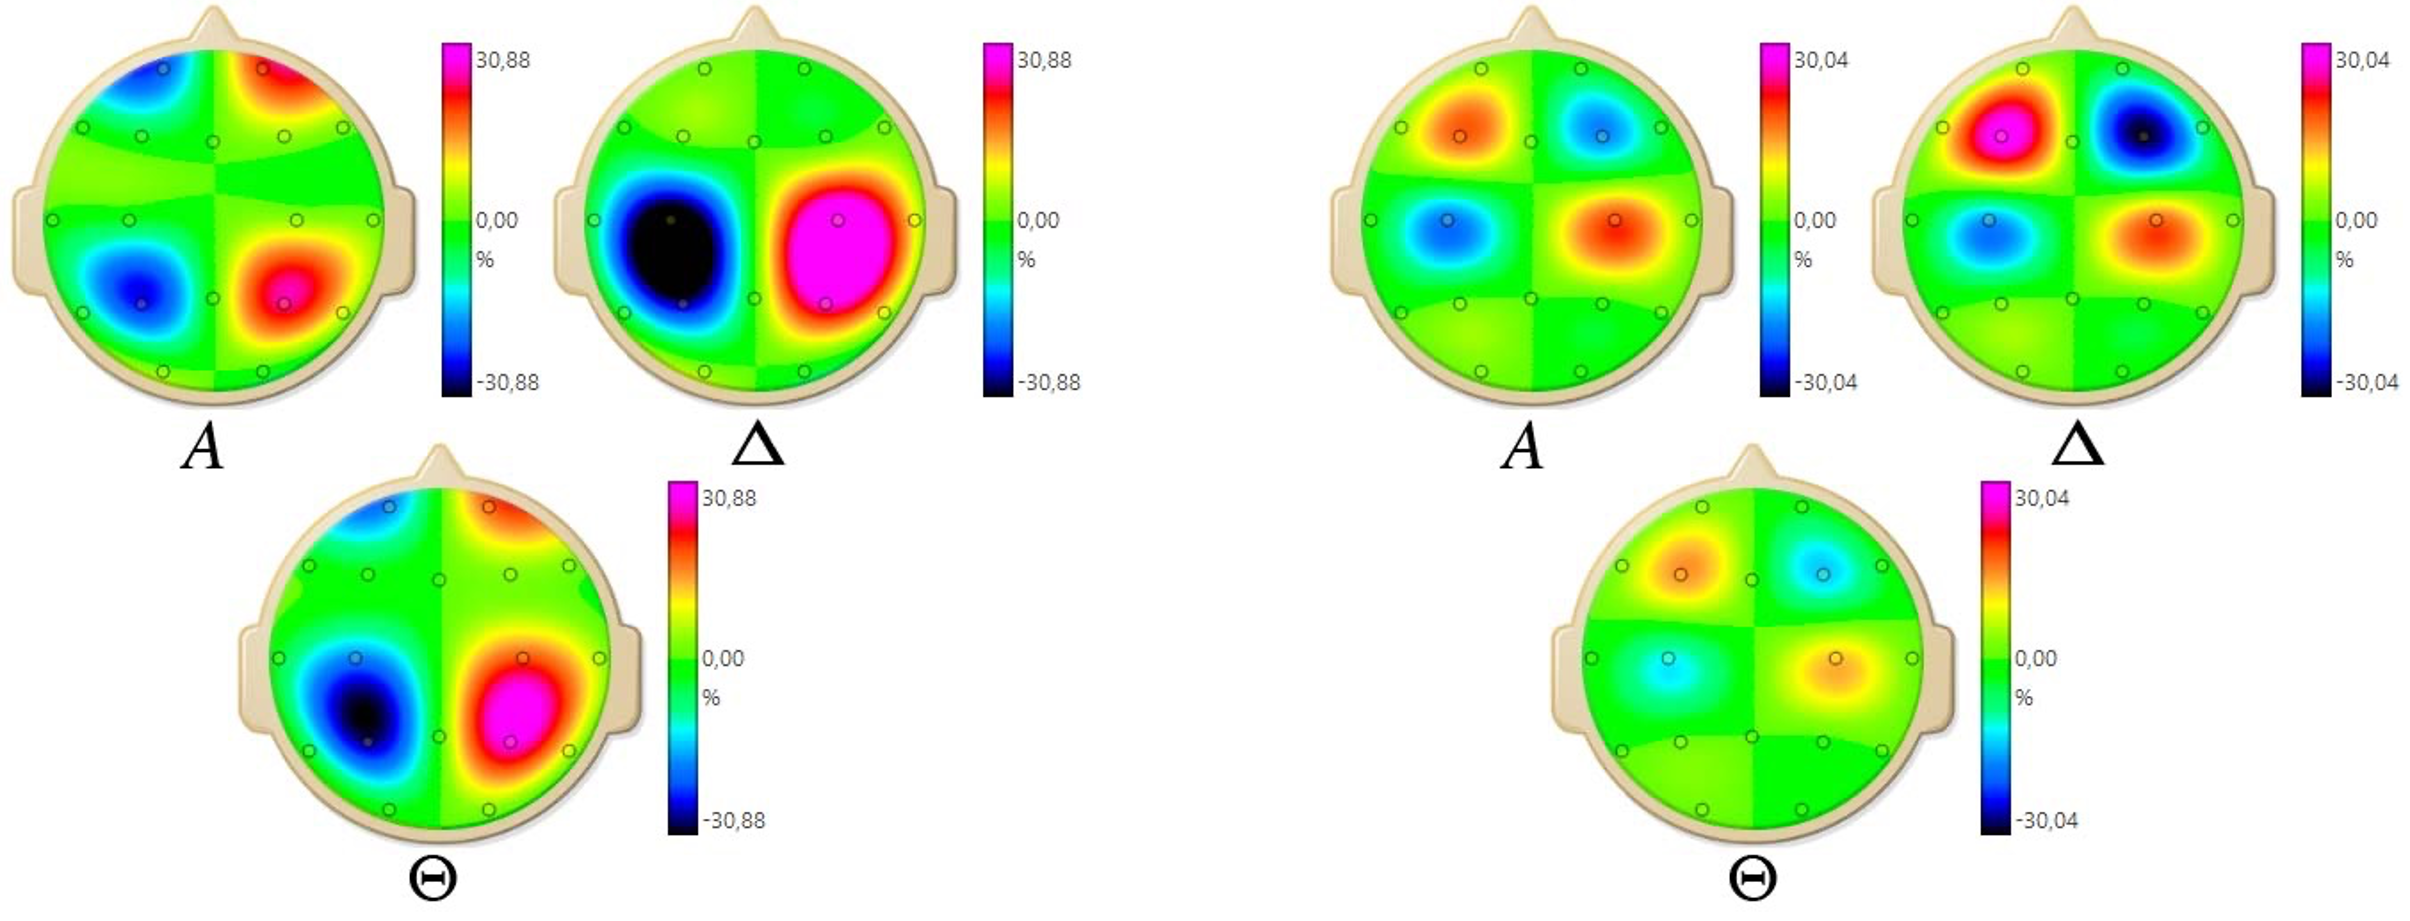
\includegraphics[width=\textwidth]{A2022.IDSEPC.ConcettoDiSoftware/SoftwareAttoCreativoEEG.png}
\end{center}

\end{frame}

\begin{frame}
{\centerline{Sentir ...  (2/3)}}
\begin{itemize}
    \item Il software \`{e} simile ad altri risultati di creazioni umane
\end{itemize} 
\begin{center}
    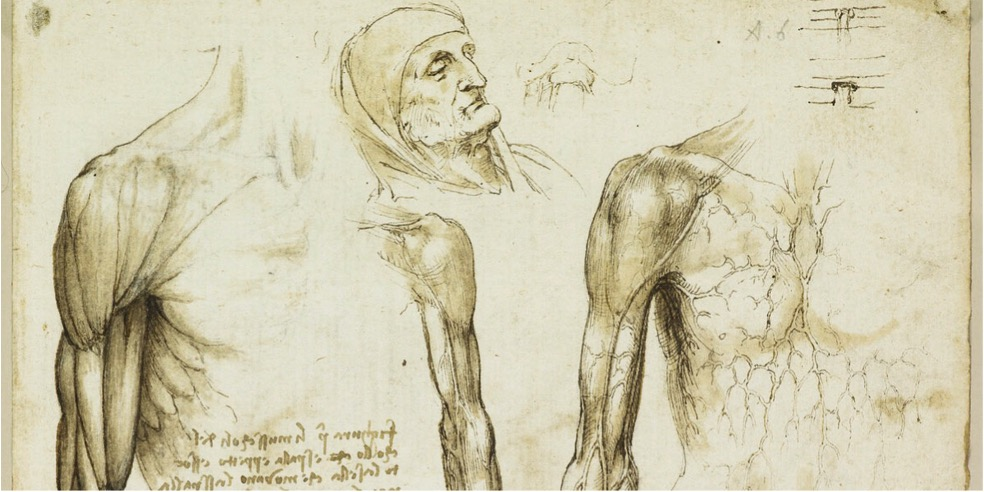
\includegraphics[width=\textwidth]{A2022.IDSEPC.ConcettoDiSoftware/SoftwareAttoCreativoLeonardo.jpg}
\end{center}

\end{frame}

\begin{frame}
{\centerline{Sentir ...   (3/3)}}
\begin{itemize}
    \item Il software \`{e} protetto dal diritto d'autore (anche se la questione \`{e} sempre aperta)
\begin{itemize}
    \item I diritti degli sviluppatori sono divisi in diritti morali (non alienabili) e diritti economici (alienabili)
    \item I diritti dei creatori sono protetti anche se non registrano un brevetto 
    \item I diritti durano molto pi\`{u} a lungo di quelli di un brevetto -- 50 anni dopo la morte del creatore invece che 20 anni dopo la registrazione del brevetto 
    \item Il software \`{e} dato in licenza e non venduto
\end{itemize} 
\end{itemize} 

\end{frame}

\begin{frame}
{\centerline{Meditar}}
\begin{center}
    \begin{tikzpicture}[scale=0.9]
\begin{axis}[
axis x line=center,
axis y line=center,
xmin = -0.95,
xmax = 9.95,
ymin = -0.95,
ymax = 11,
title={Costo marginale per unit\`{a}},
xlabel = {Numero di unit\`{a} prodotte},
yticklabels={,,},
extra x ticks = {0},
extra x tick label = {$\hspace{-0.6cm}0$},
]
\addplot[very thick,domain=0.01:0.94,samples=100,red] {0.040*x/(ln(x)^2)};
\addplot[very thick,domain=0.94:1.06,samples=10,red] {0.040*0.94/(ln(0.94)^2)};
\addplot[very thick,domain=1.06:10,samples=100,red] {0.032*x/(ln(x)^2});
\addplot[very thick,dotted] coordinates {(1,0) (1,10)};
\addplot[thick,dashed,green] coordinates {(0,10) (10,10)};
\end{axis}
\end{tikzpicture}
\end{center}

\end{frame}

\begin{frame}
{\centerline{La segmentazione del mercato nel software}}
\begin{itemize}
\item Nel software non ci sono limiti fisici alla segmentazione
\item Inoltre:
\begin{itemize}
\item il software \`{e} protetto dal copyright
\item la funzione di costo ha una struttura a ``L''
\end{itemize}
\item Si pu\`{o} quindi operare un segmentazione aggressiva
\item Si possono operare strategie di ``bundling'' per promuovere nuovi prodotti
\end{itemize}

\end{frame}

\begin{frame}
{\centerline{Esempio di segmenti di mercato}}

\begin{itemize}
    \item Questi dati sono molto vecchi, ma il succo non cambia:
\end{itemize}

\begin{center}
    
\resizebox{0.9\textwidth}{!}{%
  \begin{tabular}{|c|c|c|c|}
  \hline
  \textbf{Prodotto} & \textbf{Professional} & \textbf{Educational} & \textbf{E/P} \\
  \hline
    Office 97 & \$ 779 & \$ 215.45 & 27.6\% \\ \hline
    Corel WP Suite 98 & \$ 449 & \$ 71.55 & 15.9\% \\
  \hline
  \end{tabular}

} % end of scope of "\resizebox"  directive
\end{center}
\end{frame}

\begin{frame}
{\centerline{Altro esempio di segmentazione (16/09/2022)}}
\begin{center}
    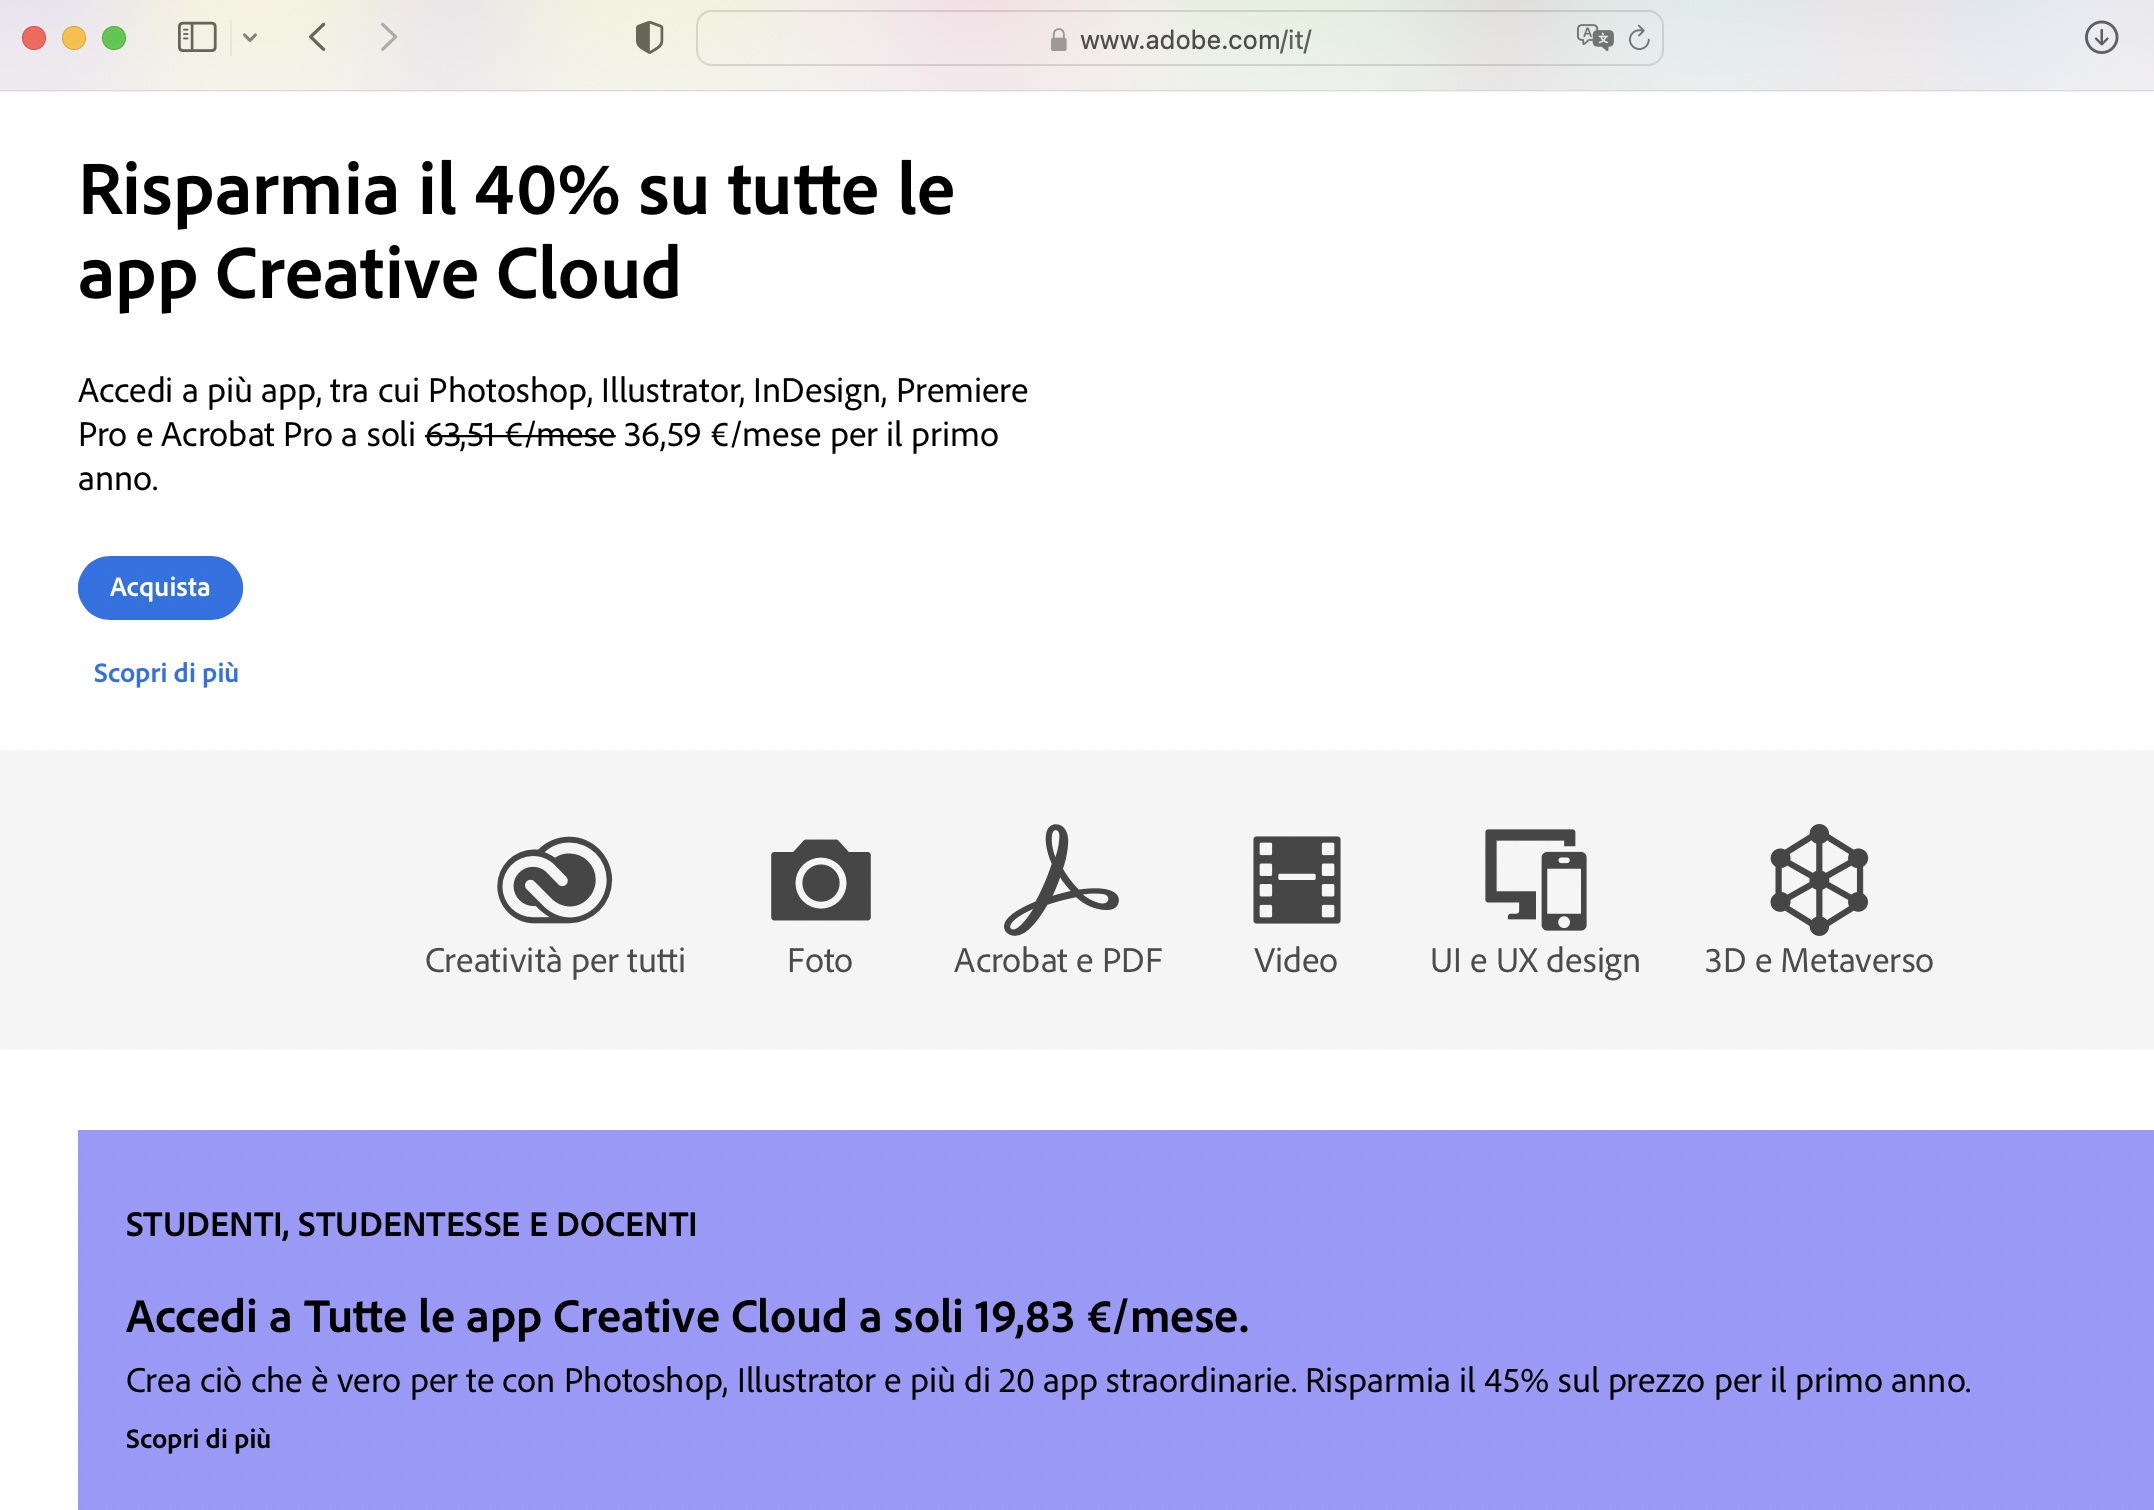
\includegraphics[width=0.8\textwidth]{A2022.IDSEPC.ConcettoDiSoftware/SegmentationBundlingAdobe.jpg}
\end{center}

\end{frame}

\begin{frame}
{\centerline{Bundling (16/09/2022)}}
\begin{center}
    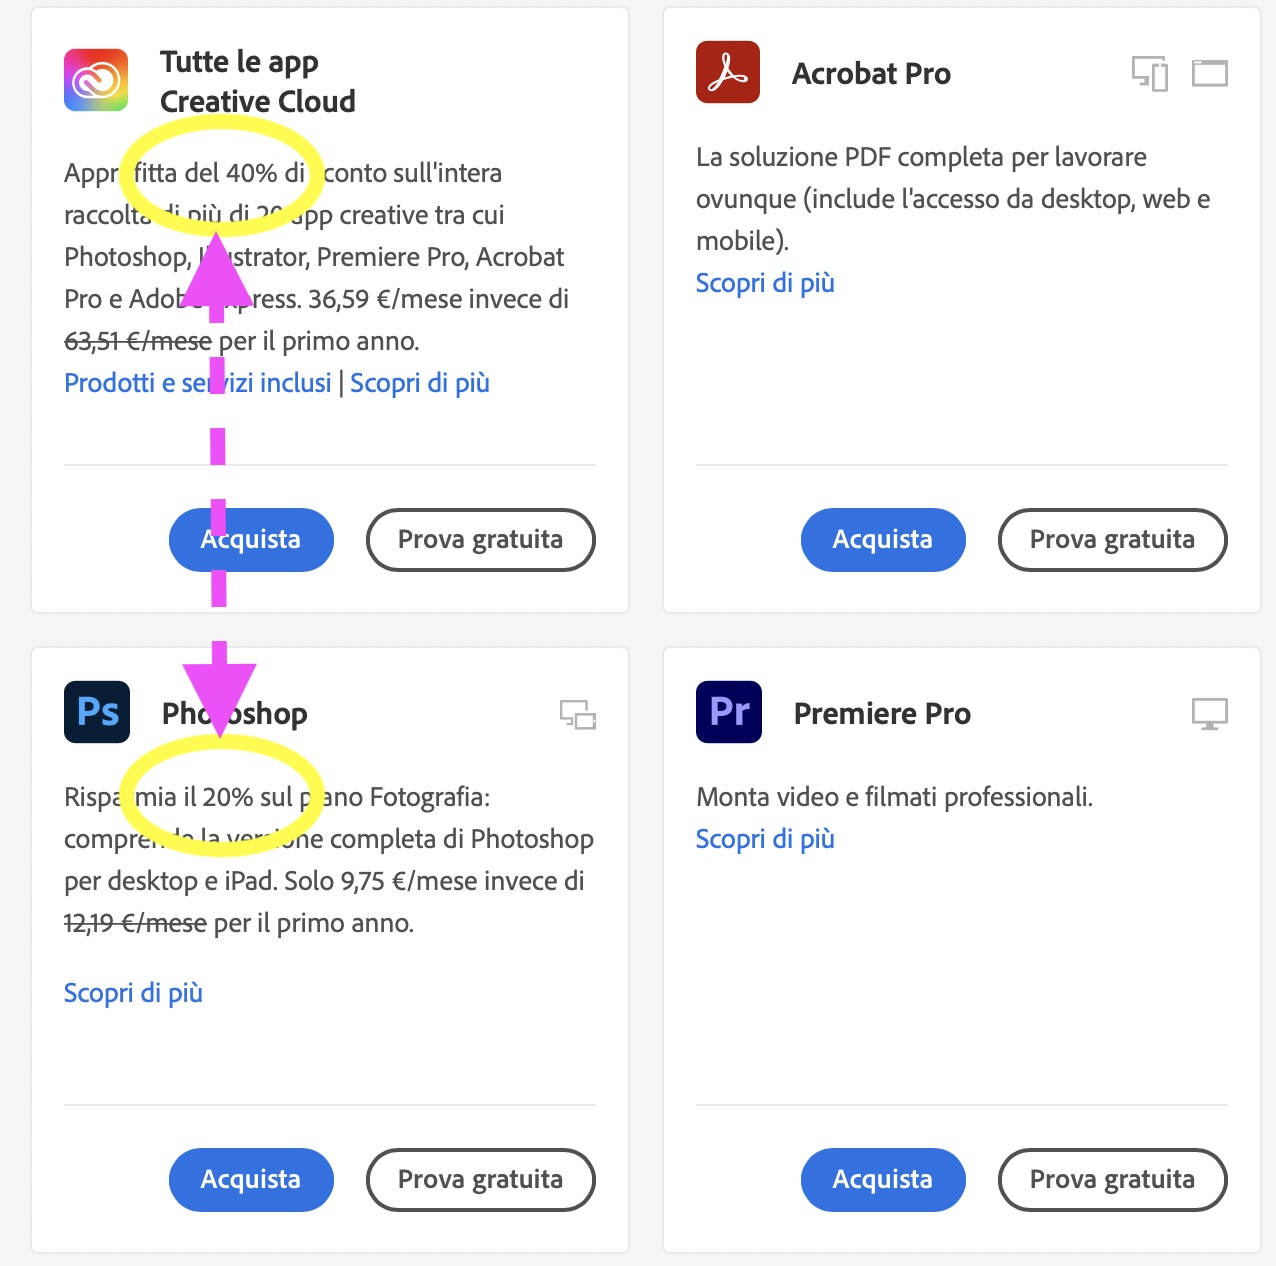
\includegraphics[width=0.6\textwidth]{A2022.IDSEPC.ConcettoDiSoftware/BundlingAdobe.jpg}
\end{center}

\end{frame}

\begin{frame}
{\centerline{Bundling in altri settori ``creativi'' (1/2)}}
\begin{center}
    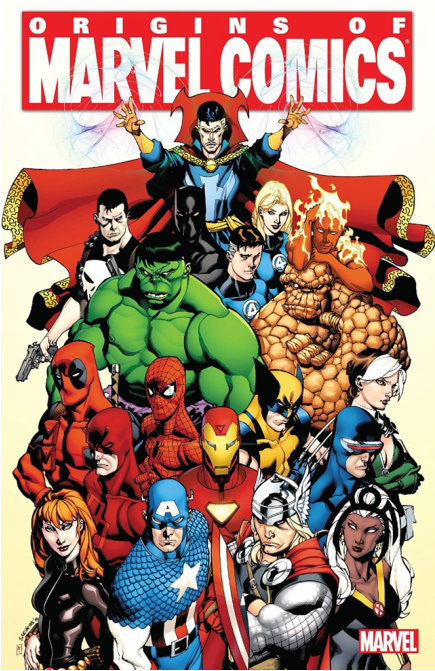
\includegraphics[width=0.4\textwidth]{A2022.IDSEPC.ConcettoDiSoftware/BundlingMarvel.pdf}
\end{center}

\end{frame}

\begin{frame}
{\centerline{Bundling in altri settori ``creativi'' (2/2)}}
\begin{center}
    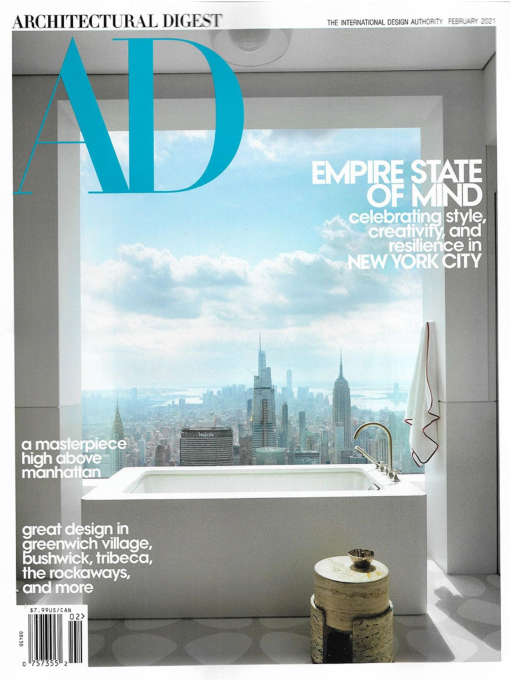
\includegraphics[width=0.45\textwidth]{A2022.IDSEPC.ConcettoDiSoftware/BundlingAD.pdf}
\end{center}

\end{frame}

\begin{frame}
{\centerline{Programmar(e)}}
       \begin{tabular}{lc}  
       \begin{tabular}{l}
             \parbox{0.4\linewidth}{%  change the parbox width as appropiate
             \begin{itemize}
                \item Raccontare storie $\ldots{}$ perch\'{e}?
                \item Scrivere software, cio\`{e} programmare, \`{e} come raccontare storie
                \item Italo Calvino ci insegna:
                \begin{itemize}
                    \item Leggerezza
                    \item Rapidit\`{a}
                    \item Esattezza
                    \item Visibilit\`{a}
                    \item Molteplicit\`{a}
                \end{itemize}
                \item Non \`{e} il primo
            \end{itemize}

             }
         \end{tabular} &
         \begin{tabular}{c}
           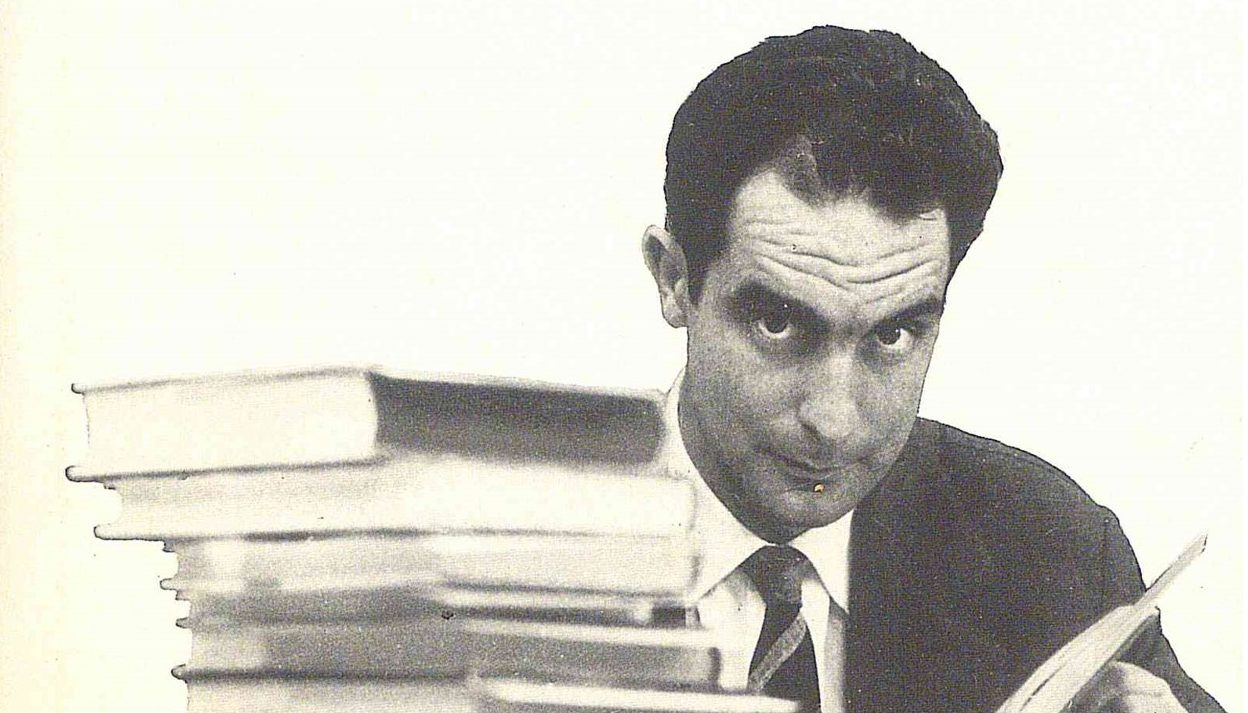
\includegraphics[width=.5\textwidth]{P2023.SentirMeditarEProgrammar.Pillola/Calvino5.jpg}
           \end{tabular}
       \end{tabular}
\end{frame}


\begin{frame}
{\centerline{Catone}}

\begin{figure}[htp]
    \centering
     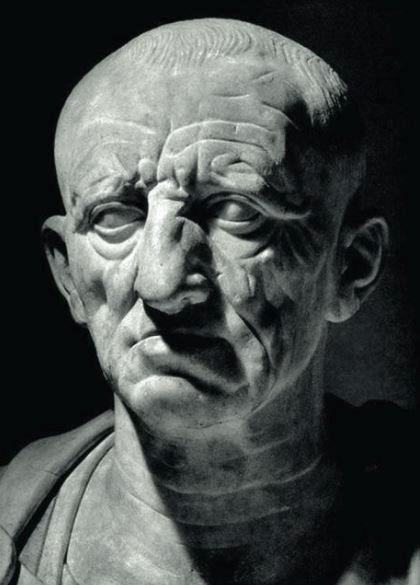
\includegraphics[width=.32\textwidth]{P2023.SentirMeditarEProgrammar.Pillola/CatoneIlCensore.jpg}
    \label{F:CatoneIlCensore}
\end{figure}

\begin{center}
    \Large{\textcolor{red}{Rem tene,} \textcolor{blue}{verba sequentur!}}\\
    \textit{Che cosa ci insegna nella programmazione?}
\end{center}
\end{frame}



\begin{frame}
{\centerline{Cicerone}}

       \begin{tabular}{cl}  
         \begin{tabular}{c}
           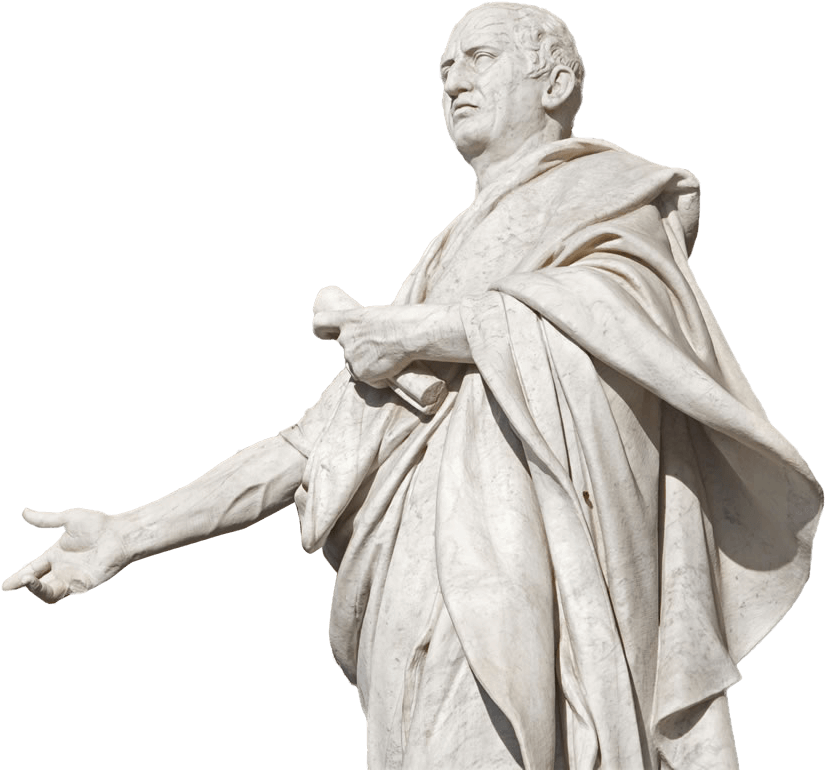
\includegraphics[width=.5\textwidth]{P2023.SentirMeditarEProgrammar.Pillola/Cicero.png}
           \end{tabular}
           & \begin{tabular}{l}
             \parbox{0.5\linewidth}{%  change the parbox width as appropiate
             \Large
             \begin{itemize}
                \item Inventio
                \item Dispositio
                \item Elocutio
                \item Memoria
                \item Actio
             \end{itemize}

            }
         \end{tabular}
       \end{tabular}

\end{frame}

\begin{frame}
{\centerline{Dante}}

       \begin{tabular}{cl}  
         \begin{tabular}{c}
           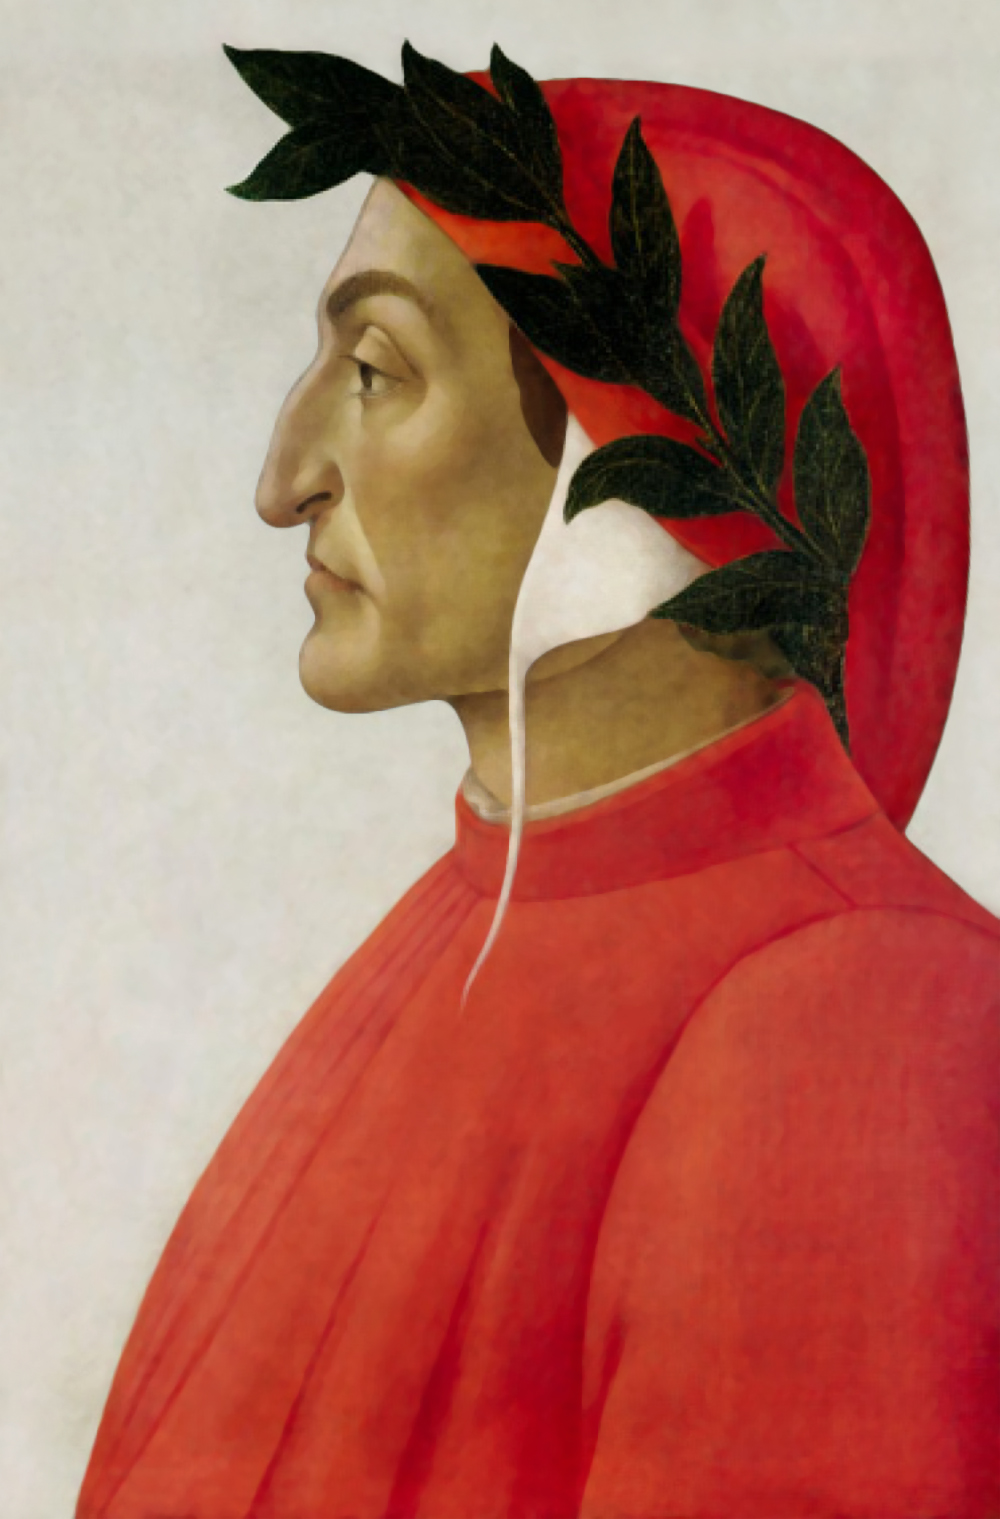
\includegraphics[width=.35\textwidth]{P2023.SentirMeditarEProgrammar.Pillola/Dante.jpg}
           \end{tabular}
           & \begin{tabular}{l}
             \parbox{0.6\linewidth}{%  change the parbox width as appropiate
            E io a lui: ``I' mi son un che, quando\\
            Amor mi spira, noto, \textcolor{red}{\bf e a quel modo}\\
            ch'e' ditta dentro vo significando.''
            }
         \end{tabular}
       \end{tabular}

\end{frame}

\begin{frame}
{\centerline{Italo Calvino: un maestro}}

       \begin{tabular}{cl}  
         \begin{tabular}{c}
           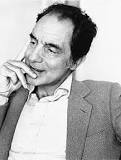
\includegraphics[width=.4\textwidth]{P2023.SentirMeditarEProgrammar.Pillola/Calvino.jpg}
           \end{tabular}
           & \begin{tabular}{l}
             \parbox{0.5\linewidth}{%  change the parbox width as appropiate
             \begin{itemize}
                \item Cuba, 1923 -- Italia 1985
                \item Scrittore, giornalista, sistemico
                \item Visitatore sia di Russia/URSS e USA
            \end{itemize}

             }
         \end{tabular}
       \end{tabular}

\end{frame}

\begin{frame}
{\centerline{Il lavoro di Italo Calvino}}

       \begin{tabular}{cl}  
         \begin{tabular}{c}
           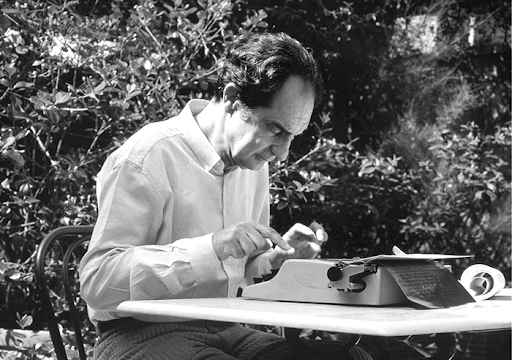
\includegraphics[width=.4\textwidth]{P2023.SentirMeditarEProgrammar.Pillola/Calvino2.png}
           \end{tabular}
           & \begin{tabular}{l}
             \parbox{0.5\linewidth}{%  change the parbox width as appropiate
             \begin{itemize}
                \item Ispirato dai ciberneti e dai primi informatici
                \item Ha persino cercato di creare storie da combinazioni di situazioni
                \item Grande attenzione alla semantica delle parole e delle frasi come collezioni di parole
            \end{itemize}

             }
         \end{tabular}
       \end{tabular}

\end{frame}


\begin{frame}
{\centerline{L'opera di nostro interesse }}

       \begin{tabular}{cl}  
         \begin{tabular}{c}
           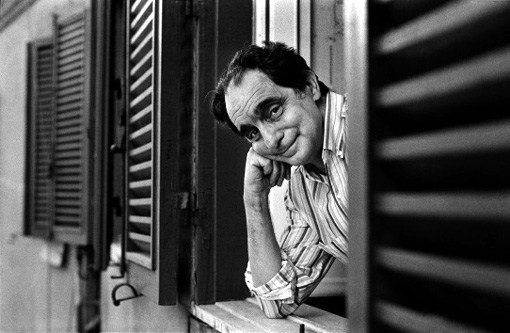
\includegraphics[width=.4\textwidth]{P2023.SentirMeditarEProgrammar.Pillola/Calvino3.jpg}
           \end{tabular}
           & \begin{tabular}{l}
             \parbox{0.5\linewidth}{%  change the parbox width as appropiate
             \begin{itemize}
                \item Scrisse (senza completarle) ``Lezioni americane. Sei proposte per il prossimo millennio''
                \item  6 lezioni che si sarebbero dovute tenere a Harvard 
                \item Ci\`{o} che il terzo millennio dovrebbe imparare dal secondo nella scrittura
            \end{itemize}

             }
         \end{tabular}
       \end{tabular}

\end{frame}

\begin{frame}
{\centerline{Struttura dell'opera (di nuovo)}}

       \begin{tabular}{cl}  
         \begin{tabular}{c}
           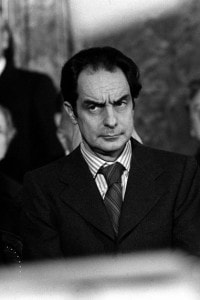
\includegraphics[width=.4\textwidth]{P2023.SentirMeditarEProgrammar.Pillola/Calvino4.jpg}
           \end{tabular}
           & \begin{tabular}{l}
             \parbox{0.5\linewidth}{%  change the parbox width as appropiate
             \begin{itemize}
                \item Leggerezza
                \item Rapidit\`{a}
                \item Esattezza
                \item Visibilit\`{a}
                \item Molteplicit\`{a}
                \item \textit{[ Coerenza ]}
            \end{itemize}
             }
         \end{tabular}
       \end{tabular}

\end{frame}


\begin{frame}
{\centerline{Domande?}}
\vspace{1cm}
\begin{center}
    \LARGE{Fine della pillola.}
\end{center}

\end{frame}


\end{document}
